\documentclass{article}

\usepackage[a4paper]{geometry} % document dimensions
\usepackage{amsmath} % multiline equation numbering
\usepackage{amssymb} % e.g. triangleq, checkmark
\usepackage{textcomp,gensymb} % \degree symbol
%\usepackage{bm} % bold symbols numbering
\usepackage{authblk} % author/affiliation block
\usepackage[T1]{fontenc} % support accents via UTF
\usepackage[titletoc,title]{appendix}
\usepackage{booktabs} % e.g. \toprule
\usepackage{pdflscape} % e.g. roatate tables _and_ display rotated

\usepackage{graphicx} % support for graphics
\usepackage[hidelinks, backref=page]{hyperref} % hyperlinks and autoref
\hypersetup{
    pdfauthor={Nick Ackerley},
    pdfsubject={Engineering Seismology},
    pdftitle={An Open Model of Probabilistic Seismic Hazard Assessment for the Indian Subcontinent},
    pdfkeywords={seismology, hazard, India, OpenQuake}}
\usepackage{natbib} % bibliography support
\usepackage{adjustbox} % support for too-wide figures
\usepackage{caption} % support for captions of floats
\usepackage{capt-of} % support for captionof
\usepackage{subcaption} % support for multiple figures with captions
\providecommand*\hyphen{-} % dashed page numbers in bib
\usepackage{listingsutf8} % for syntax-highlighted code
\usepackage[usenames,dvipsnames]{xcolor} % e.g. RoyalBlue
\usepackage{fontspec} % support for setmonofont
\setmonofont{Ubuntu Mono}[Scale=MatchUppercase]

%\usepackage{multirow} % cells spanning rows in \crefs
%\usepackage{array} % vertically aligned table cells

\usepackage{enumitem} % control list formatting
\setlist{noitemsep}

% allow figures to take up more of a page
\renewcommand{\floatpagefraction}{0.7}

% just call everything a "section", except an "appendix"
\renewcommand*{\sectionautorefname}{Section}
\renewcommand*{\subsectionautorefname}{Section}
\renewcommand*{\subsubsectionautorefname}{Section}
\newcommand*{\Appendixautorefname}{Appendix}

% set up back-references
\renewcommand*{\backref}[1]{}
\renewcommand*{\backrefalt}[4]{%
    \ifcase #1 (Not cited.)%
    \or        (Cited on page~#2.)%
    \else      (Cited on pages~#2.)%
    \fi}

\lstdefinelanguage{Ini}
{
    basicstyle=\ttfamily\footnotesize,
    breaklines=true,
    keepspaces=true,
    columns=fullflexible,
    morecomment=[s][\color{RoyalBlue}\bfseries]{[}{]},
    morecomment=[l]{\#},
    morecomment=[l]{;},
    commentstyle=\color{gray}\ttfamily,
    morekeywords={},
    otherkeywords={=,:},
    keywordstyle={\color{green}\bfseries},
}

%%% PREAMBLE

\begin{document}

\section{Under what conditions is it permissible to collapse magnitude-frequency distributions?}

In classical PSHA the hazard integral gives an estimate of rate at which the ground motion $Y$ at a site of interest will exceed some value $y$. For a set of $N_S$ sources generating ruptures of $N_M$ magnitudes $m_j$ at $N_R$ distances $r_k$ using discrete summations,  \citep{baker2008introduction}:

\begin{equation} \label{eq:HazardIntegral} 
\lambda(Y > y) = 
\sum_{i=1}^{N_S} 
\lambda(M_i > m_\text{min}) 
\sum_{j=1}^{N_M} 
\sum_{k=1}^{N_R} 
P_i(Y > y|m_j,r_k) 
P_i(M_i=m_j) 
P_i(R_i=r_k)
\end{equation}

Where for source $i$:
\begin{itemize}
\item $\lambda_i(M_i > m_\text{min})$ is the rate of earthquakes greater than $m_\text{min}$
\item $P_i(Y > y|m_j,r_k)$ is the ground motion prediction equation (GMPE) and incorporates aleatory uncertainty in the ground motion
\item $P_i(M_i=m_j)$ is the frequency-magnitude distribution (FMD)
\item $P_i(R_i=r_k)$ is the distribution of distance measures from points within the source to the site of interest.
\end{itemize}

For a single point source, neglecting finite source effects, this simplifies to:

$$ \lambda(Y > y) = 
\lambda(M > m_\text{min}) 
\sum_{j=1}^{N_M} 
P(Y > y|m_j,R) 
P(M=m_j) $$

But now suppose that certain epistemic uncertainties have been identified. In order to estimate the effect of this lack of knowledge on the mean and spread of ground motions suppose $N_G$ GMPEs $P_\ell(Y > y|m_j,R)$ have been assigned weights $w_\ell$ and $N_F$ FMDs $P_m(M=m_j)$ have been assigned weights $w_m$. Now

$$ \lambda(Y > y) = 
\lambda(M > m_\text{min}) 
\sum_{m=1}^{N_F} w_m 
\sum_{\ell=1}^{N_G} w_\ell 
\sum_{j=1}^{N_M} 
P_\ell(Y > y|m_j,R) 
P_m(M=m_j) $$

Since we can reorder the summations to obtain

$$ \lambda(Y > y) = 
\lambda(M > m_\text{min}) 
\sum_{\ell=1}^{N_G} w_\ell 
\sum_{j=1}^{N_M} 
P_\ell(Y > y|m_j,R) 
\sum_{m=1}^{N_F} w_m 
P_m(M=m_j) $$

We can pre-compute the ``collapsed'' FMD for the source:

$$ P_C(M=m) \equiv \sum_{m=1}^{N_F} w_m P_m(M=m) $$

And this simplifies the hazard summation to

$$ \lambda(Y > y) = 
\lambda(M > m_\text{min}) 
\sum_{\ell=1}^{N_G} w_\ell 
\sum_{j=1}^{N_M} 
P_\ell(Y > y|m_j,R) 
P_C(M=m_j) $$

Note that a similar ``collapse'' of GMPE uncertainty is not possible because the ground motion is conditional upon the magnitude.

\begin{figure}[!htb]
\begin{adjustbox}{center}
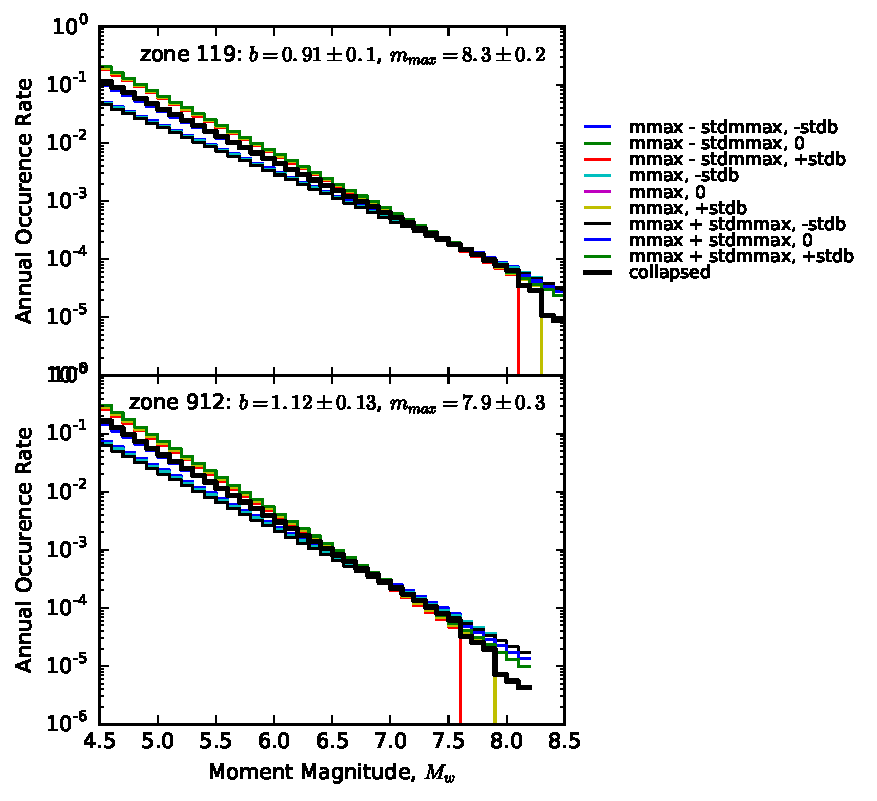
\includegraphics{Mean_Occurrence_Rates_Zones_119_912}
\end{adjustbox}
\caption[Frequency-magnitude distributions for two zones nearest to Guwahati, India]{Frequency-magnitude distributions corresponding to various branches of the logic tree of \cite{nath2012probabilistic}. The zones chosen are the two closest to Guwahati, India. Zone 119 at 25-50 km depth is the zone capable of producing a devastating ``pop-up'' type event \citep{Bilham2001, nath2012ground}. The ``collapsed'' FMD uncertainty computed using \eqref{eq:CollapsedFmd} is shown as a heavy black line.} 
\label{fig:CollapsedFmd}
\end{figure}

This analysis says that collapsed FMDs should give an exact result for the mean exceedance rate. \autoref{fig:MeanFullVsCollapsed} shows that collapsing FMDs gives a very good approximation of the mean hazard for low probabilities of exceedance but not for high. It is not yet clear to me why this should be the case; it may relate to the choice of return period or to the magnitude bin width. 

\begin{figure}[!htb]
\begin{adjustbox}{center}
\includegraphics{Guwahati_mean_Zones_119_912}
\end{adjustbox}
\caption[Mean hazard curves computed using various levels of FMD uncertainty]{Mean hazard curves computed using various levels of FMD uncertainty. The site of interest is the city of Guwahati. The source model consists only of zones 119 and 912 of \cite{nath2012probabilistic}. The full GMPE logic tree of \cite{nath2012probabilistic} is used. The ``fully enumerated'' result implements the FMD logic tree described in \cite{nath2012probabilistic} while ``collapsed'' implements \eqref{eq:CollapsedFmd} and ``no FMD uncertainty'' models only the FMD logic tree branches with the largest weights.} 
\label{fig:MeanFullVsCollapsed}
\end{figure}

Returning to the case of multiple sources, we can include ground-motion and frequency-magnitude epistemic uncertainty by writing:

$$ \lambda(Y > y) = 
\sum_{i=1}^{N_S} 
\lambda_i(M_i > m_\text{min}) 
\sum_{m=1}^{N_F} w_{m,i} 
\sum_{\ell=1}^{N_G} w_{\ell,i}
\sum_{j=1}^{N_M} 
\sum_{k=1}^{N_R} 
P_{\ell,i}(Y > y|m_j,r_k) 
P_{m,i}(M_i=m_j) 
P_i(R_i=r_k) $$

We can still reorder the summations, as long as we recognize that the collapsed FMD is different for each source

$$
\lambda(Y > y) = 
\sum_{i=1}^{N_S} 
\lambda(M_i > m_\text{min}) 
\sum_{\ell=1}^{N_G} w_{\ell,i}
\sum_{j=1}^{N_M} 
\sum_{k=1}^{N_R} 
P_{\ell,i}(Y > y|m_j,r_k) 
P_i(R_i=r_k) 
\sum_{m=1}^{N_F} w_{m,i} 
P_{m,i}(M_i=m_j) 
$$

So that for source $i$ the collapsed FMD is

\begin{equation} \label{eq:CollapsedFmd} 
P_{Ci}(M_i = m) \equiv
\sum_{m=1}^{N_F} w_{m,i} 
P_{m,i}(M_i=m) 
\end{equation}

The important point here is that the ``collapsed'' FMD can be pre-computed for each source. In an application with $N_S$ sources, if there are $3^2$ branches to the FMD logic tree this means $3^{2 N_S}$ branches can be eliminated in all. In a simple example with a single site, two areal sources and a moderately complex GMPE logic tree (see \autoref{fig:MeanFullVsCollapsed}) computation time on a quad-core laptop dropped from 36 minutes to 55 seconds when FMD uncertainty was collapsed. In mapping type applications with gridded sites and hundreds of areal sources, each with FMD uncertainty, the computational savings can make an intractable problem tractable. 

\begin{figure}[!htb]
\begin{adjustbox}{center}
\includegraphics{Guwahati_median_Zones_119_912}
\end{adjustbox}
\caption[Median hazard curves computed using various levels of FMD uncertainty]{Median hazard curves computed using various levels of FMD uncertainty. For detailed description see \autoref{fig:MeanFullVsCollapsed}} 
\label{fig:MedianFullVsCollapsed}
\end{figure}

It is my understanding that the hazard integral \eqref{eq:HazardIntegral} computes the mean hazard. It is not clear to me at the moment how quantile hazards are computed, but I will speculate using common sense. 

Aleatory variability is modelled in most if not all GMPEs using a log-normal distribution so the ability to compute an arbitrary quantile of ground-motion exceedance is built-in. 

With epistemic variability it is less clear how quantiles are computed. OpenQuake computes the exceedance probabilities for each realization separately. In some cases, with large numbers of sources, each having FMD uncertainty, OpenQuake founders simply in enumerating the possibilities. The next step must be to sort the results by probability of exceedance. Finally quantiles are located with reference to the weighting scheme. If I am correct, if there are 3 FMD branches for a source, then whichever produces the largest probability of exceedance at a given level of ground motion will determine the probability of exceedance for any percentile from the 67\textsuperscript{th} through the 100\textsuperscript{th}. Furthermore, if there are no other logic trees, for GMPEs or source models, then in fact the 67\textsuperscript{th} will be the same as the 100\textsuperscript{th} percentile hazard curve.

If this is correct, then it is obvious why the ``collapse'' of FMDs produces different results for quantile hazard curves. With the FMD logic trees collapsed the ground motions for different realizations are no longer computed and cannot be sorted, as required to find a quantile of interest. The result is just plain wrong, farther from the true result than if no FMD uncertainty is considered at all, as shown in \autoref{fig:MedianFullVsCollapsed}.

In conclusion, the collapse of FMD logic trees by weighted summation of branches is safe and gives significant reduction in computational complexity if only the mean hazard curve is of interest. In practice the mean hazard is slightly underestimated for annual probabilities of exceedance below approximately 10\%. Further investigation is needed to find out what determines this threshold; if it is dependent on the return period chosen alone then inaccuracy at low-probability of exceedance is effectively a computational artefact, a curiosity of no engineering significance. Another possibility is that it is a result of the discretisation of the FMD used; in this case it would be possible to reduce the error by discretise the FMDs using bin widths of say 0.01 magnitude units instead of 0.1, but there would be a corresponding computational penalty.

\bibliographystyle{apalike}
\bibliography{/home/nick/Desktop/Library/PSHA.bib,/home/nick/Desktop/Library/india-hazard.bib}

\end{document}